%%%%%%%%%%%%%%%%%%%%%%%%%%%%%%%%%%%%%%%%%
% University/School Laboratory Report
% LaTeX Template
% Version 3.1 (25/3/14)
%
% This template has been downloaded from:
% http://www.LaTeXTemplates.com
%
% Original author:
% Linux and Unix Users Group at Virginia Tech Wiki 
% (https://vtluug.org/wiki/Example_LaTeX_chem_lab_report)
%
% License:
% CC BY-NC-SA 3.0 (http://creativecommons.org/licenses/by-nc-sa/3.0/)
%
%%%%%%%%%%%%%%%%%%%%%%%%%%%%%%%%%%%%%%%%%

%----------------------------------------------------------------------------------------
%	PACKAGES AND DOCUMENT CONFIGURATIONS
%----------------------------------------------------------------------------------------

\documentclass{article}

\usepackage[version=3]{mhchem} % Package for chemical equation typesetting
\usepackage{siunitx} % Provides the \SI{}{} and \si{} command for typesetting SI units
\usepackage{graphicx} % Required for the inclusion of images
\usepackage{natbib} % Required to change bibliography style to APA
\usepackage{amsmath} % Required for some math elements 
\usepackage[utf8]{inputenc}
\usepackage{tikz,pgfplots}
\usepackage[letterpaper, margin=0.5in]{geometry}
\usepackage{float}
\usepackage{enumitem}
\usepackage{gensymb}
\usepackage[hidelinks]{hyperref}
\usepackage[all]{hypcap}
\usepackage{subfloat}
\usepackage{color}
\usepackage{listings}

% Roman numerials
\pagenumbering{arabic}

\setlength\parindent{0pt} % Removes all indentation from paragraphs

%\renewcommand{\labelenumi}{\alph{enumi}.} % Make numbering in the enumerate environment by letter rather than number (e.g. section 6)

%\usepackage{times} % Uncomment to use the Times New Roman font

% for some tables
\newcommand{\specialcell}[2][c]{%
  \begin{tabular}[#1]{@{}c@{}}#2\end{tabular}}
  
\newcommand{\me}{\mathrm{e}}
\providecommand{\e}[1]{\ensuremath{\times 10^{#1}}}

\newcommand{\eqname}[1]{\tag*{#1}}

\DeclareMathOperator\erfc{erfc}

%%%%%%%%%%%% COLOR DEFINITIONS %%%%%%%%%%%%%

\definecolor{silicon}{RGB}{255,102,102}
\definecolor{oxide}{RGB}{145,150,110}
\definecolor{ioxide}{RGB}{175,180,135}
\definecolor{goxide}{RGB}{195,200,150}
\definecolor{poly}{RGB}{155,20,155}
\definecolor{spinglass}{RGB}{200,205,100}
\definecolor{n+}{RGB}{250,15,15}
\definecolor{aluminum}{RGB}{30,30,30}

%----------------------------------------------------------------------------------------
%	DOCUMENT INFORMATION
%----------------------------------------------------------------------------------------

%\title{Determination of the Atomic \\ Weight of Magnesium \\ CHEM 101} % Title

%\author{John \textsc{Smith}} % Author name

%\date{\today} % Date for the report

\begin{document}

%\maketitle % Insert the title, author and date

% If you wish to include an abstract, uncomment the lines below
% \begin{abstract}
% Abstract text
% \end{abstract}

%----------------------------------------------------------------------------------------
%	SECTION 1
%----------------------------------------------------------------------------------------

\section{Profiles \& Layout}
\subsection{}
\subsection{}
\subsection{}
\section{Process Procedures}
\subsection{}
\subsection{}
\subsection{}
\section{Calculations}
a) Film Thickness
\begin{figure}[H]
\centering
\begin{tabular}{c || c | c | c | c | c | c}
Layer & \specialcell{Theoretical \\ calculation \\ (nm)} & \specialcell{Experimental \\ (nm)} & \% Error & \specialcell{Linewidths \\ (photoresist) \\ (nm)} & \specialcell{Linewidths \\ (after PR Strip) \\ (nm)} & \% Overetch \\ \hline

Field Oxide & 505.8 & 477.2 & 5.65 & ? & 3000 & ? \\ \hline
Polysilicon & ? & ? & ? & ? & ? & ? \\ \hline
Gate Oxide & 80.1 & 86.5 & 7.40 & 3628 & 4000 & ? \\ \hline
Intermed Oxide & 386.3 & 320 & 17.2 & ? & ? & ? \\ \hline
Aluminum & 800 & ? & ? & 2088 & 2520 & ? \\ \hline

\end{tabular}
\end{figure}

b) Sheet Resistance 
\begin{figure}[H]
\centering
\begin{tabular}{c || c | c }
Layer & \specialcell{Sheet Resistance \\ (??)} & \specialcell{Surface concentration \\ (??)} \\ \hline

\specialcell{ACTV after \\ Field Oxidation} & ? & ? \\ \hline
Polysilicon & ? & ? \\ \hline
\specialcell{ACTV after \\ Pre-Dep} & ? & ? \\ \hline
\specialcell{ACTV after \\ Drive-In} & ? & ? \\ \hline
Metal & ? & ? \\ \hline

\end{tabular}
\end{figure}

c) Overetch
\begin{figure}[H]
\centering
\begin{tabular}{c || c | c | c | c | c}
Layer & \specialcell{Measured Linewidth \\ (nm)} & \% Overetch & \specialcell{Theoretical \\ etch time \\ (min)} & \specialcell{Actual \\ etch time \\ (min)} & \% Overetch \\ \hline

Field Oxide &  ? & ? & 4.8 & 6 & 25 \\ \hline
Polysilicon &  ? & ? & 1.6 & $\sim2.25$ & 41  \\ \hline
Gate Oxide &  ? & ? & 0.87 & ? & ? \\ \hline
Intermed Oxide &  ? & ? & 3.2 &  4.5 & 41 \\ \hline
Aluminum &  ? & ? & 1.4 & $\sim5$ & 360 \\ \hline

\end{tabular}
\end{figure}
%%%%%%%%%%%%%%%%%%%%%%%%%%%%%%
\begin{description}[style = nextline]
\item[1) Theoretical and experimental thicknesses of field oxide, gate and intermediate 
oxides (Include orientation dependence of oxidation rate but not impurity 
dependence) (9 points)]
For details on the theoretical oxide thickness calculations see Appendix \textcolor{blue}{\ref{sec:oxide}}.
%NOTE REDO DRY OXIDE AND INCLUDE TAO OF 25nm!
\begin{figure}[H]
\centering
\begin{tabular}{c || c | c | c}
Layer & \specialcell{Theoretical \\ (nm)} & \specialcell{Experimental \\ (nm)} & \% Error \\ \hline
Field Oxide & 505.8 & 477.2 & 5.65 \\ \hline
Gate Oxide & 80.1 & 86.5 & 7.40  \\ \hline
Intermed Oxide & 386.3 & 320 & 17.2 \\ \hline
\end{tabular}
\end{figure}

\item[2) Junction depths after pre-diffusion and drive-in (theoretical, assume only 
phosphorous doping with surface concentration limited by solid solubility). You 
must consider the effect of the initial ion implantation. For pre-deposition you may 
use the box approximation, but for drive-in you must use the half-gaussian 
calculation. Why is this? (10 points)]

For details on the junction depth calculations see Appendix \textcolor{blue}{\ref{sec:jdepth}}. Also the reason we use a box approximation for the pre-diffusion is because we have a constant source profile. However, for drive-in we now have source-limited diffusion.

\begin{figure}[H]
\centering
\begin{tabular}{c || c}
Step & \specialcell{Junction Depth \\ (nm)} \\ \hline
Pre-diffusion & 365 \\ \hline
Drive-in & 1000 \\ \hline
\end{tabular}
\end{figure}

\item[3) test]
test

\item[4) Plot or sketch the change of dopant profile from the silicon surface through the source-drain after each thermal step. Quantitatively label significant points such as Peak concentration, Peak Width, Junction Depth. Show movement of the Silicon-Silicon Dioxide interface and qualitatively show non-ideal effects such as dopant redistribution during oxidation. (11 points)]
The profiles were all created in Tsuprem-4 using the EE143 process flow.

\begin{itemize} 
\item Field Oxidation 
\end{itemize}
\begin{figure}[H]
\centering
\begin{tikzpicture}
\node at (5,5) {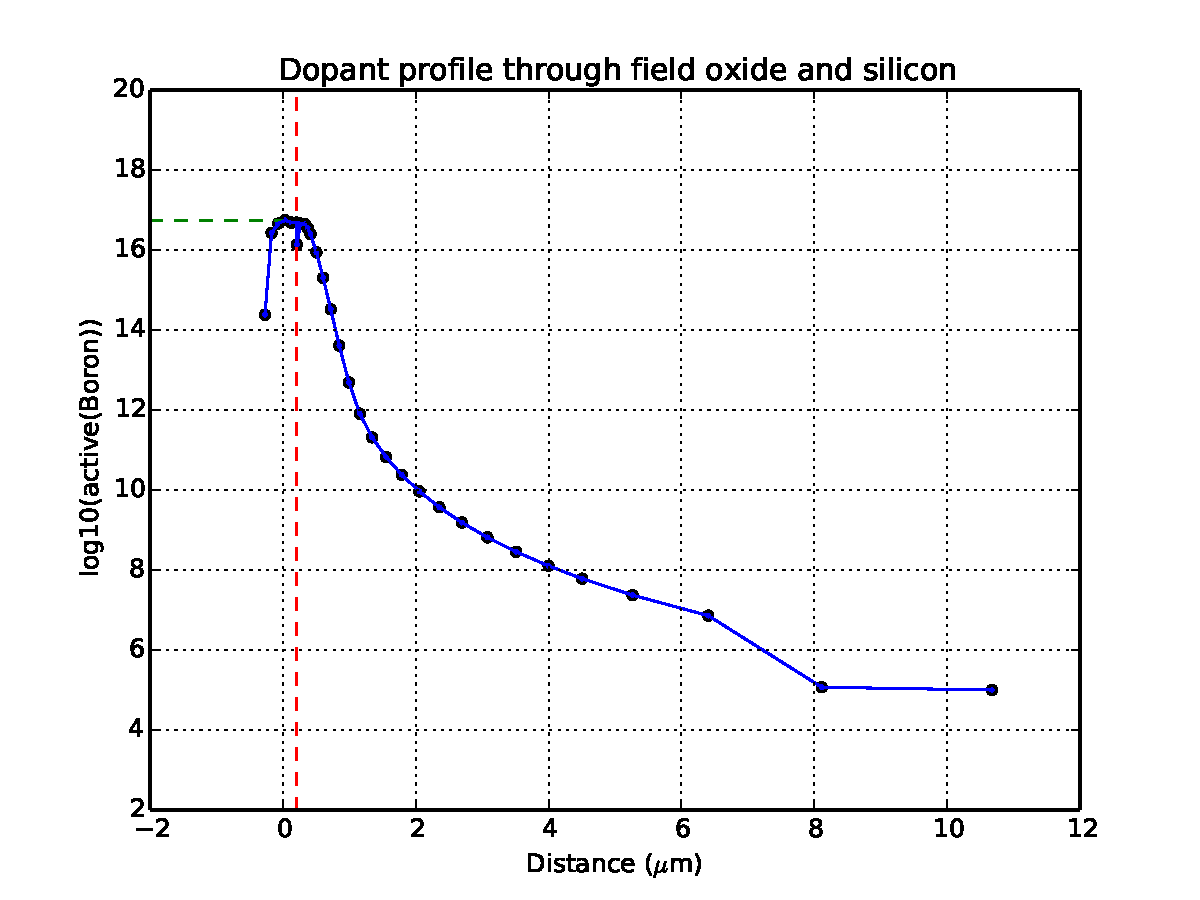
\includegraphics[width=350pt]{dope_profile/profile1.pdf}};
\node at (1.1,2.5) {\textbf{Si$\text{O}_2$}};
\node at (2.5,2.5) {\textbf{Si}};
\node at (1.0,7.6) {16.74};
\end{tikzpicture}
\caption{Dopant profile with only field oxide. The Si-Si$\text{O}_2$ interface occurs at 0.2104$\mu$m. There was about 500 nm of field oxide deposited here. The peak concentration is roughly ${10}^{16.74}$.}
\label{fig:doping1}
\end{figure}

\begin{itemize} 
\item Gate Oxidation 
\end{itemize}

\item[5) test]
test

\item[6) List an estimate of the Young's modulus, Poisson ratio, and coefficient of thermalexpansion for Si$\text{O}_2$, poly-Si, and Al films as deposited. (You can find these in a table in many physics/ME textbooks, or in a web-based search.) (2 points) ]
See table below

\begin{figure}[H]
\centering
\begin{tabular}{c || c | c | c}
Material & \specialcell{Young's modulus \\ (GPa)} & \specialcell{coeff. of \\ thermal expansion \\ ($K^{-1}$)} & \specialcell{Poisson's ratio \\ (a.u.)} \\ \hline
Si$\text{O}_2$ [3]& 57(dry)-70(wet) & 5.6 $ \cdot$ 10$ ^{-7}$  & 0.17 \\ \hline
poly-Si [2]& 169 $\pm$ 6.15 & 4.6 $ \cdot$ 10$ ^{-6}$ & 0.22 $\pm$ .011 \\ \hline
Aluminum [4]& 70 & 22.2 $\cdot$ 10$ ^{-6}$ & 0.33 \\ \hline
\end{tabular}
\caption{Values were found from various journals/articles found online ([2],[3], and[4]) and many of these values are calculated for thin films of the material.}
\end{figure}


\end{description}
\section{Questions}
\begin{description}[style = nextline]
\item[1) What type of photoresist (positive or negative? I-line or G-line?) do we use in the
lab? What do I-line and G-line refer to? Briefly describe how the resist responds
to the process steps like spinning, UV light exposure and development.]

\item[2) What is the purpose of baking the wafers at 120 $\degree$C before depositing HMDS? What
is the purpose of the 90 $\degree$C bake after spinning on photoresist? What happens if the
soft bake is too hot and too long (say 120 $\degree$C, 5 minutes)?]

\item[3) What is the purpose of hard bake? What happens if we skip this step? What may
happen if the bake is done at a temperature above 120 $\degree$C (say 200 $\degree$C)?]

\item[4) We do lithography steps under yellow light only. What is the consequence if we
expose the wafers to fluorescent light before development? What if we expose
them to fluorescent light after development? Would red light damage your process?]

\item[5) What are the differences between wet and dry oxidation that lead us to use one for
the gate oxide and one for the field/intermediate oxide? What is the purpose of
annealing in nitrogen after oxidation?]

\item[6) How do you determine etching time using theoretical etch rate in literature? List
two ways to determine etch time empirically from lab measurements, when you
etch the layers. (Hint: these methods include visual cues.). How close are the
experimental and the theoretically calculated values?]

\item[7) Before n+ deposition (prior to SOG spinning), we clean in Piranha but not in HF.
Before gate oxidation, we clean in both. Why the difference?]

\item[8) Why is 5:1 BHF (5:1 N$\text{H}_4$F:HF) used for etching features in the oxide while 10:1
BHF is used for cleaning and spin-on-glass stripping? Why buffered HF? ]

\item[9) What would happen if we skipped the HF dip before metallization? ]

\item[10) What is etch selectivity? ]

\item[11) Why do we first use the roughing pump and then the diffusion pump when pumping
down the aluminum deposition system? Why must the foreline pressure be kept
below 100 mTorr?]

\item[12) What is the Al etchant composed of? What happens if you use it at room
temperature? What is the purpose of sintering? What will result if sintering step is
skipped? What happens if sintering temperature is too hot or too low?]


\item[13) Briefly explain the mechanism of Xe$\text{F}_2$ etching. Is the etch isotropic or
anisotropic? In an integrated CMOS/MEMS process, is there any consequence to
using KOH instead of Xe$\text{F}_2$ for etch?]

\item[14) . What would happen if a thick oxide film was left on the wafers as it went into the
Xe$\text{F}_2$ etching step? ]

\item[15) Identify two of the 11 major processing steps that are unnecessary to fabricate a
functional oxide cantilever beam. Why are they unnecessary?]

\end{description}






\section{Appendix}

\subsection{Oxide Thickness calculations}
\label{sec:oxide}
Film thickness calculation for oxides:
\begin{equation}
X_{ox} = \frac{0.5B}{B/A}\Big[\sqrt{1 + \frac{4}{B}(\frac{B}{A})^2(t + \tau)} - 1\Big]
\end{equation}
\begin{equation}
\tau = \frac{{X_i}^2}{B} + \frac{X_i}{B/A}
\end{equation}
where
\begin{align*}
B/A = D_o\me^{\frac{-E_a}{kT}} (\text{Use table 3.1 [1] to find }E_a \text{and } D_o) \\
B = D_o\me^{\frac{-E_a}{kT}} (\text{Use table 3.1 [1] to find }E_a \text{and } D_o) \\
t = \text{Time of oxide growth} \\ 
\tau = \text{Time of initial oxide growth already present} \\
X_i = \text{length of initial oxide growth}
\end{align*}

Example: Calculated oxide thickness of Intermed Oxide: \\
Given: 5 min dry oxidation at $1050\degree$C and 12 + 25 min wet oxidation annealing at $1050\degree$C, calculate oxide growth. \\

First we consider the 5 min dry oxidation. Using table 3.1 [1] for a $<100>$ Silicon, and using dry oxidation, we see that for the linear rate constant (B/A), $E_A = 2.00$ eV and $D_o = 3.71\e{6} \, \mu$m/hr. For the parabolic rate constant (B), $E_A = 1.23$ eV and $D_o = 772\, \mu$m/hr. \\ \\
Using an arrhenius equation where $k =$ Boltzmann's constant, and $T = $ temperature. 
\begin{align*}
B/A &= D_o\me^{\frac{-E_A}{kT}} = 3.71\e{6}\me^{\frac{-2.00*1.602\e{-19}}{1.38\e{-23}(1050\degree\text{C} + 273)}} = 0.0887 \mu\text{m/hr} \\
B &= D_o\me^{\frac{-E_A}{kT}} = 772\me^{\frac{-1.23*1.602\e{-19}}{1.38\e{-23}(1050\degree\text{C} + 273)}} = 0.0159 \,{\mu\text{m}}^2\text{/hr}
\end{align*}
Since there is no initial oxide here, $\tau = 0$,
\begin{align*}
X_{ox} = \frac{0.5B}{B/A}\Big[\sqrt{1 + \frac{4}{B}(\frac{B}{A})^2(t + \tau)} - 1\Big] = \frac{0.5 (0.0159)}{0.0887}\Big[\sqrt{1 + \frac{4}{0.0159}(0.0887)^2(\frac{5\text{min}}{60\text{min/hr}} + 0)} - 1\Big] \approx 7.11 \, \text{nm}
\end{align*}

Now after this dry oxidation, we have a 37 minute wet oxidation at $1050 \degree$C. Using table 3.1 [1] again, but this time using the constants that apply for wet oxidation,

\begin{align*}
{B/A}_{\text{wet}} &= D_o\me^{\frac{-E_A}{kT}} = 9.70\e{7}\me^{\frac{-2.05*1.602\e{-19}}{1.38\e{-23}(1050\degree\text{C} + 273)}} = 1.50 \mu\text{m/hr} \\
B_{\text{wet}} &= D_o\me^{\frac{-E_A}{kT}} = 386\me^{\frac{-0.78*1.602\e{-19}}{1.38\e{-23}(1050\degree\text{C} + 273)}} = 0.411 \,{\mu\text{m}}^2\text{/hr}
\end{align*}

This time we do have an initial oxidation time $\tau$ because of the dry oxidation we did in the previous step. Here $X_i$ is the oxide length we calculated for the dry oxidation growth,

\begin{align*}
\tau = \frac{{X_i}^2}{B_{\text{wet}}} + \frac{X_i}{{B/A}_{\text{wet}}} = \frac{0.00711^2}{0.411} + \frac{0.00711}{1.50} \approx 0.00488 \text{hrs}
\end{align*}

And finally our oxide growth is,
\begin{align*}
X_{ox} = \frac{0.5B}{B/A}\Big[\sqrt{1 + \frac{4}{B}(\frac{B}{A})^2(t + \tau)} - 1\Big] = \frac{0.5 (0.411)}{1.50}\Big[\sqrt{1 + \frac{4}{0.411}(1.50)^2(\frac{(12 + 25)\text{min}}{60\text{min/hr}} + 0.00488 \text{hrs})} - 1\Big] \approx 386.3 \, \text{nm}
\end{align*}

\subsection{Junction Depth Calculations}
\label{sec:jdepth}
Junction depth calculation for box approximation (limited-source diffusion):
\begin{equation}
x_j = 2\sqrt{Dt \ln{(N_o/N_B)}}
\end{equation}
and for a half gaussian (constant-source diffusion):
\begin{equation}
x_j = 2\sqrt{Dt}\erfc^{-1}{(N_B/N_o)}
\end{equation}
where,
\begin{align*}
D &= D_o\me{\frac{-E_A}{kT}} \,\,\text{(Diffusion coefficient)} \\ 
t &= \text{time of diffusion} \\
N_B &= \text{Background impurity concentration} \\ 
N_o &= \text{Surface concentration limited by solid solubility}
\end{align*}

Example: Calculate the junction depth after pre-diffusion and drive in. \\
According to the process flow [5], our silicon wafer has a resistivity of about 14-16 ohm-cm. From the same process flow we know that we had a phosphorus doped, solid solubility limited constant diffusion at $1050\degree$C. Using figure 4.6 [1] we see that at a temperature of $1050\degree$C our phosphorus surface concentration $N_o \approx 10^{21}$/$\text{cm}^3$. Now using the Resistivity of our wafer and figure 4.8 [1], we see that we have an impurity concentration $N_B \approx 8\e{14}/\text{cm}^3$. \\ \\
Using table 4.1 [1], we can calculate our diffusion coefficient. Note that pre-diffusion was done at $1050\degree$C for 5 minutes.
\begin{align*}
D &= D_o\me{\frac{-E_A}{kT}} = 10.5 \,\text{cm}^2/\text{sec}\,\, \exp{(\frac{-3.69*1.602\e{-19}}{1.38\e{-23}(1050 + 273)})} = 9.11\e{-14} \, \text{cm}^2/\text{sec}
\end{align*}
Now we can plug everything into our solid solubility limited box approximation equation:
\begin{align*}
x_j = 2\sqrt{Dt}\erfc^{-1}{(N_B/N_o)} = 2\sqrt{(9.11\e{-14})(300\text{sec})} \erfc^{-1}{(8\e{14}/10^{21})} \approx 365 \,\text{nm}
\end{align*}

Now for drive-in we kept the temperature the same, $1050\degree$C, but kept the wafer inside the furnace for 37 minutes (2220 seconds). Also we can no longer assume a simple box approximation, we must use a half gaussian; this means that our surface concentration is going to change with drive-in. \\\\
We will use the following equation,

\begin{equation}
N_B = (Q/\sqrt{\pi D_2t_2})\exp{(-(\frac{x_j}{2\sqrt{D_2t_2}})^2)}
\end{equation}

where Q is the does rate,
\begin{equation}
Q = 2N_o\sqrt{D_1t_1/\pi}
\end{equation}

Combining the two equations and noting that $D_1 = D_2$ because we are using the same temperature, $1050\degree$C, for both pre-diffusion and drive-in ($t_1$ is the pre-diffusion time and $t_2$ is the drive in time),

\begin{align*}
N_B = (2N_o/\pi)\sqrt{\frac{t_1}{t_2}}\exp{(-(\frac{x_j}{2\sqrt{D_2t_2}})^2)}
\end{align*}
Solving this for $x_j$ yields,
\begin{align*}
x_j = 2\sqrt{D_2t_2\ln{\big((2N_o/\pi N_B)(\sqrt{t_1/t_2})\big)}} = 2\sqrt{(9.11\e{-14})(2220)\ln{\big((2(10^{21})/\pi (8\e{14}))(\sqrt{300/2220})\big)}} \approx 1000 \,nm
\end{align*}

\subsection{Dopant Profiles.}
\begin{itemize}
\item Field Oxide
\end{itemize}
According to the EE143 process flow, There was an initial blanket implant of B11 3E12$\text{cm}^{-3}$ on our $<100>$ wafer. Also our wafer had a resistivity of 14-16cm which corresponds to a background concentration of about 8E14$\text{cm}^{-3}$. Now for the field oxide, we used 5-80-5 minute dry,wet,dry oxidation to create about 500 nm of oxide. Putting all this information into Tsuprem-4 generates the plot in Figure \textcolor{blue}{\ref{fig:doping1}}. \\ \\
Script file: 
\begin{verbatim}
$ field oxide

$ Initialization 
Initialize <100> material=silicon Phosphorus=8e14 width=1.5 dX=0.005

$ Blanket implant here
Implant B11 Energy=60 Dose=3e12

$ 5-80-5 oxidation
Diffusion Time=5 Temperature=1000 DryO2
Diffusion Time=80 CONTINUE Temperature=1000 WetO2
Diffusion Time=5 CONTINUE Temperature=1000 DryO2

$ plotting
Select z=log10(active(boron))
Plot.1d
Print.1d
\end{verbatim}

\begin{itemize}
\item Gate Oxide
\end{itemize}



%----------------------------------------------------------------------------------------
%	SECTION 5
%----------------------------------------------------------------------------------------
\section{References}
\begin{enumerate}
\item Jaeger, Richard. \textit{Introduction to microelectronic fabrication}. New Jersey: Prentice Hall, 2002. Print.
\item Sharpe, William N., Bin Yuan, and Ranji Vaidyanathan. Measurements of Young's Modulus, Poisson's ratio, and Tensile Strength of Polysilicon. Publication no. 1. Nagoya: IEEE, 1997. Web.
\item Kim, Min. "Influence of Substrates on the Elastic Reaction of Films for the Microindentation Tests." Thin Solid Films 283 (1996): 15. Web.
\item Chinmulgund, M. "Effect of Ar Gas Pressure on Growth, Structure, and Mechanical Properties of Sputtered Ti, Al, TiAl, and Ti3Al Films." Thin Solid Films 270.1-2 (1995): 260-63. Web.
\end{enumerate}

%----------------------------------------------------------------------------------------
%	SECTION 6
%----------------------------------------------------------------------------------------

% Nothing right now

%----------------------------------------------------------------------------------------
%	BIBLIOGRAPHY
%----------------------------------------------------------------------------------------

\bibliographystyle{apalike}

\bibliography{sample}

%----------------------------------------------------------------------------------------


\end{document}

